\documentclass[letterpaper,twoside,onecolumn,openright,final]{memoir}
%    vs.       others...   oneside twocolumn openleft  draft showtrims
%                          twoside onecolumn openany   ms
%                                            openright final 
\input lumos_common
\begin{document}
\frontmatter

\thispagestyle{empty}
\ThisLLCornerWallPaper{1}{images/cover}
%\strut 
\vfill
\begin{center}
{\HUGE Assembling the Lumos\TM}

\bigskip

{\HUGE 24-Channel DC Controller}

\vfill

\end{center}

\newpage
\begin{center}
\LLimg[width=1in]{danger-generic}

%DANGER! 

\mc{RISK OF FIRE, ELECTROCUTION, SERIOUS INJURY OR DEATH!} 
\end{center}

This circuit design, including but not limited to any associated plans, schematics, designs, board layouts, documentation, 
and/or components, is \mc{EXPERIMENTAL} and for \mc{EDUCATIONAL} purposes only. It is not a finished consumer-grade product.
It is assumed that you have the necessary understanding and skill to assemble and/or use electronic circuits.

Proceed \mc{ONLY} if you know exactly what you are doing, understand the proper procedures for working with the high voltage present on the components and PC boards, and understand that you do so \mc{ENTIRELY AT YOUR OWN RISK.}

The author makes \mc{NO} representation as to suitability or fitness for any purpose whatsoever, and disclaims any and all liability or warranty to the full extent permitted by applicable law.
\index{warranty, limitation of}
\index{danger warnings}
\index{warnings}

\strut\vfill
\noindent Edition 1.0, for Lumos 24-Channel DC Controller circuit version 1.0.8.

\smallskip


\noindent Copyright \copyright\ 2013 by Steven L. Willoughby,
Aloha, Oregon, USA.  All Rights Reserved.  
This document is released under the terms and conditions of the 
Creative Commons ``Attribution-NoDerivs 3.0 Unported'' license.  
In summary, you are free to use, reproduce, and redistribute this 
document provided you give full attribution to its author and do not
alter it or create derivative works from it.  See
\URL{http://creativecommons.org/licenses/by\-nd\-/\-3.0/} for the full
set of licensing terms.

\begin{center}
\LLimg[width=.5in]{cc}\LLimg[width=.5in]{by}\LLimg[width=.5in]{nd}
\end{center}

\newpage
\tableofcontents

\mainmatter

\chapter{Introduction}
\LLstart{C}{ongratulations}{on joining} the many computer-controlled
Christmas light enthusiasts, \ix{theatrical lighting} technicians, electronics hobbyists,
\index{Christmas lights}
and home automation innovators who are experimenting with new ways to have computers
control lights and other electronic devices.

The Lumos\TM\ 24-Channel DC Controller board places 24 such devices under the control
of your computer.  These outputs are arranged into three \ix{blocks} of eight \ix{channels}.
Each block is electrically isolated from the logic control circuit and from each other,
so each block may be separately powered at different voltages if desired.

If Lumos boards are configured with the \ix{RS-485} network option, up to sixteen Lumos
boards may be ``daisy chained'' together (a total of 384 channels) and controlled from 
the same PC serial port.
By plugging DC-powered Christmas lights into the Lumos controller, your PC can orchestrate
a dazzling display of lights synchronized to music.

This manual details the process of assembling a Lumos controller from a bare printed
circuit board and set of components, and also shows the various optional configurations
which may be used during construction.

\section{Intended Audience}
This is an ``advanced'' level do-it-yourself electronic circuit project.  It is not
an off-the-shelf consumer-ready product.  It is only designed for educational and experimental
use by experienced hobbyists and professionals who possess the skill to construct electronic
\marginpar{\centerline{\LLimg[height=.5in]{danger-sign}}}
circuits, to understand how they function, troubleshoot problems with them, and to use them safely.

\section{Limitation of Warranty}
\index{danger warnings}
\index{warnings}
\index{warranty, limitation of}
Since this is a do-it-yourself project, the quality of the final product, and whether it 
functions as intended, is largely a result of your own efforts in building it.  As such, we
cannot offer to troubleshoot, repair, or replace a board we did not assemble for you.  Accordingly,
\marginpar{\centerline{\LLimg[height=.5in]{danger-sign}}}
these instructions, and all accompanying plans, schematics, software, hardware, and other
project materials are provided to you ``\mc{AS-IS}'' at no cost, as a courtesy between 
\acronym{DIY} hobbyists with \mc{NO WARRANTY} of any kind expressed or implied.  If you proceed
to build and/or use this unit, you do so \mc{ENTIRELY AT YOUR OWN RISK}.

If you purchased hardware materials from us (such as a PC board or programmed controller chip),
we will---at our sole discretion---replace, repair, or refund the cost of those materials if they were defective in manufacture
as shipped to you, up to 90~days from the date they were shipped to you,
but are not liable for damage caused by your handling or assembly of the unit.
Otherwise, we make no representation of suitability or fitness for any particular purpose and disclaim
all other warranty or liability of any kind to the full extent permitted by law.

\section{How to Use this Manual}
Please begin by reviewing the safety information in Chapter~\ref{ch:safety}.  

When you are ready to begin assembling your Lumos controller, gather the required tools and materials
as explained in Chapter~\ref{ch:materials}.  

Then read carefully the \emph{entire} set of instructions in the following chapters
beginning any actual work.  Begin assembly \emph{only} if you understand all the steps you will need
to carry out.

Once your controller is complete and ready to use, refer to the separate manual,
\emph{Using Lumos SSR Controllers} for full instructions on how to program
and use your controller with your computer or in stand-alone operation.

\section{The Name of the Game}
The name ``Lumos'' is a combination of \emph{lumen}, the Latin word for ``light,''
and the initial letters of ``Orchestration System.''  Hence, ``Light Orchestration System''
which is the most common application for which the Lumos hardware and software are used---running
computerized lighting displays.

\section{Getting Additional Help}
The \ix{product website} at \URL{www.alchemy.com/lumos} contains additional documentation,
\index{website}
pointers, hints, and tips to assist you further.  If that doesn't answer all your questions,
there is an \ix{online forum} where you may submit questions for help.


\chapter{Safety Information}\label{ch:safety}

\LLstart{B}{efore}{you begin building} your Lumos controller, please take the time to
carefully read the following \ix{safety precautions}.  Failure to follow this advice could
result in death or serious injury, damage to the Lumos controller unit, and/or damage
to the other devices plugged into the controller.
\index{danger warnings}
\index{warnings}

\section{Hazardous Materials}
While assembling this unit you may come in contact with \ix{hazardous chemicals}.  The Lumos
product contains no hazardous parts \emph{per se} but if you choose to assemble it using
lead-based solder, you may expose yourself to risk of \ix{lead poisoning}.  The main cause of lead
\marginpar{\centerline{\LLimg[height=.5in]{poison_sign}}}
poisoning due to soldering is by ingesting lead particles left on your hands or work surface.
To avoid this, keep food away from your work area, and thoroughly wash your hands and work
surfaces before handling food.

In addition, if you choose to use other chemical agents (e.g., to clean excess flux from your
soldered board), be sure to read and follow their precautions and instructions carefully.

\section{Small Part Danger}
This board contains small parts which could pose a \ix{choking hazard} to small children.
This product is not a toy and is not intended for use by children in any circumstance.
The small parts on the product can be swallowed by children under 4~years of age. Keep
\marginpar{\centerline{\LLimg[height=.5in]{danger-generic}}}
out of reach of children.

\section{Hazardous Voltage}
Exercise care when working with any electrical system, including one such as the Lumos DC
controllers (even though in theory they deal with low voltages).  The power supplies of the
loads plugged into the Lumos controller, and even the power loads being controlled, may present
\marginpar{\centerline{\LLimg[width=.5in]{danger-shock}}}
a \ix{shock hazard} if not wired and handled using standard safety protocols.  Never touch or work
with live circuits. Always disconnect the power source before working on your Lumos controller.

When working with loads outdoors, be sure all supplies are plugged into \acronym{GFIC}-protected
circuits.

\section{Physical Hazards}
While assembling the unit, always wear \acronym{ANSI}-approved \ix{eye protection} gear.  When soldering,
always be aware of---and in control of---the location of your soldering iron (it will be 300$^\circ$F--500$^\circ$F---any slight 
\marginpar{\centerline{\LLimg[height=.5in]{danger-generic}}}
mistake can be costly, painful, or dangerous)! Bits of molten metal or flux can spatter onto your
skin or in your eyes during soldering.  When cutting leads, sharp metal wires may be launched into the
air, and could hit your eyes.

\section{Electrostatic Discharge (ESD) Warning}
Many of the components used in this project are sensitive to static electricity.  Always use a proper
\acronym{ESD}-safe work environment when handling them, or these parts may be permanently damaged.  If
a part is damaged in this way, 
\marginpar{\centerline{\LLimg[height=.5in]{esd_symbol_l}}}
it is impossible to tell by looking at the part, and you won't necessarily
feel the \ix{static discharge} which caused the damage.  Never take the risk of handling sensitive components
without \acronym{ESD} protection in place.
\index{danger warnings}
\index{warnings}

These parts include all transistors (Q0--Q23), voltage regulators (U6--U8 and U11), diodes (D0--D11),
and integrated circuits (U0--U5, U9--U10, and U12--U13).

\section{Circuit Loading}
Always respect the maximum voltage and current capacity of the board and your wiring.  Overloading any
\index{overloaded circuits}
\index{maximum limits}
of these may result serious injury, death, fire, and/or severe damage to any or all of the devices in use.

Each block of eight controlled loads may not exceed 
\marginpar{\centerline{\LLimg[height=.5in]{danger-sign}}}
10\,A total for the block.  
Each single output channel
may not exceed 5\,A.  These should be considered \emph{absolute maximum} tolerances.  The board was designed
to operate at sustained levels below those limits.

\chapter{Before You Begin}\label{ch:before}
\LLstart{T}{HE}{Lumos controller} board may be built in a variety of different configurations
depending on how it will be used.  In order to know how to proceed from this point, you must
first decide what varition of Lumos board you wish to build.

\section{The Common ``Base'' Relay Configuration}

All boards
will contain 24 output relays, so our assembly instructions will begin with the step-by-step 
instructions for building this portion of the board (the entire lower half of the \acronym{PCB}).
In the bill of materials in Chapter~\ref{ch:materials}, this is listed as the ``base'' set of
materials all Lumos boards require.

You may choose to stop there, creating a remote-controllable DC relay board.  If you go this route,
you need some other circuit to provide the control (e.g., the Lumos 48-channel control board,
which can control two of these so-called ``dumb'' relays).  The control interface between them is the
26-pin connector J14, which carries +5\,V DC power to the Lumos relay board and 24 \acronym{TTL}-level
active-low logic inputs to drive the relays.


\section{The ``\acronym{CPU}'' Option (Intelligent Controller)}
If a simple ``dumb'' relay board is not what you need, then regardless of any other options selected, 
you will need to include the ``\acronym{CPU}'' option.  This includes all the control logic---including
a programmed microcontroller chip---required to make the Lumos controller an intelligent device capable
of responding to commands from a host PC or even able to act independently.

\section{Communications Options}
An intelligent board needs to have some way to communicate with the outside world.  At a minimum, it needs
to be able to receive configuration and programming commands from a host PC.  Usually, it will be fed
a live stream of commands from a PC telling it when to turn on or off various output chanels.

There are three options available for the Lumos boards:

\subsection{RS-485, Full Duplex}
RS-485 (also known as \acronym{TIA/EIA-485}) is a communications standard using differential
serial data signals in a multi-drop bus arrangement.  An RS-485 data cable may support up to 16
Lumos boards and may have a maximum length of 1,200\,m (4,000\,ft).  The cable used is unshielded
twisted pair (usually \acronym{CAT3}, \acronym{CAT5}, or \acronym{CAT6}).  

In order to use RS-485, the host PC will need some kind of \acronym{USB} or RS-232 to RS-485 adapter.

With the full duplex option, there are two independent data channels.  One is used for the host PC
to send commands to the Lumos board(s).  The other is used for the Lumos board(s) to respond back to
the host PC if asked to send status information about their configuration.


\subsection{RS-485, Half Duplex}
This option uses RS-485 as indicated above, but only a single data channel is used.  Most of the time,
the host PC keeps control of the wire and sends a stream of commands to the Lumos board(s) connected
to the wire.  However, if it asks one of them for a response, it must relinquish control of the line
and allow the Lumos board to assert control, transmit its response, then release control again.

With half-duplex operation, the PC needs to be able to control whether it asserts or releases control
of the serial data line.  The Lumos software assumes this is accomplished by switching the \acronym{DTR} 
line on when the PC is to transmit, and switching it off to release control and allow another device to
transmit.

Either RS-485 option is suitable for \acronym{DMX512} communications.

\subsection{RS-232}
RS-232 (also known as \acronym{TIA/EIA-232}) is the standard serial communications scheme used by
PCs, modems, terminals, and similar devices (although most of those functions have now been moved
to \acronym{USB} in recent years).  Since the host PC will likely either already have an RS-232
port, or can be supplied with a \acronym{USB}-to-serial adapter for less than \$15, this is the
simplest and least expensive option.

However, that simplicity comes at a price.  Only one device may be plugged in to an RS-232 line
at a time, and the cable should be a high-quality, shielded cable 25\,ft or shorter to avoid
interference which can disrupt communications.

\section{The Sensor-In Option}
Sensor inputs \index{sensors} may be added to an intelligent Lumos board to allow for external
sensors to trigger pre-programmed relay actions.  The host PC may also monitor the
sensors.

A Lumos board may accommodate up to four such sensor inputs.  These are \acronym{TTL}-level inputs
which may be active low or high (although the Lumos board provides 10\,K pull-up resistors on the
sensor input lines).  These inputs take the place of the four diagnostic \acronym{LED} indicators,
so if this route is taken those will no longer be available to assist with using the board.

\section{The Logic-Out Option}
The Lumos board provides four \acronym{TTL}-logic-level outputs \index{logic-level outputs} 
for the first four output channels.  These may be used for experimentation, diagnosis of the board,
or possibly to have one Lumos board's logic-level outputs fed into another Lumos board's sensor inputs
to coordinate their actions.

\section{Valid Option Combinations}
You need to choose one of these combinations of options to make a complete unit:
\begin{center}
    \begin{tabular}{|c|c|c|c|c|c|c|l|}\hline
	
\begin{sideways}\bfseries Base \end{sideways}
& \begin{sideways}\bfseries CPU \end{sideways}
& \begin{sideways}\bfseries FDX-485\end{sideways}
& \begin{sideways}\bfseries HDX-485\end{sideways}
& \begin{sideways}\bfseries RS-232 \end{sideways}
& \begin{sideways}\bfseries Sensor-In \end{sideways}
& \begin{sideways}\bfseries Logic-Out\quad\strut \end{sideways}
& \bfseries Description
\\\hline\hline
%	base      & CPU      & FDX      & HDX      & 232      & SI       & LO       &
	\Checkmark&          &          &          &          &          & ?        & ``Dumb'' relay-only board\\\hline
	\Checkmark&\Checkmark&\Checkmark&          &          & ?        & ?        & Full-Duplex RS-485\\\hline
	\Checkmark&\Checkmark&          &\Checkmark&          & ?        & ?        & Half-Duplex RS-485\\\hline
	\Checkmark&\Checkmark&          &          &\Checkmark& ?        & ?        & RS-232 Serial\\\hline
    \end{tabular}
\end{center}

``\Checkmark'' denotes a required option for a given configuration; ``?'' indicates an optional selection.

Note that the {\bfseries Sensor-In} and {\bfseries Logic-Out} options may be added to any of the other basic
configurations (except that {\bfseries Sensor-In} can't be used with relay-only boards).  If you don't know which option to choose, the most likely
set to be useful to begin with would either be {\bfseries Base}+{\bfseries CPU}+{\bfseries RS-232} if
you want a single Lumos board connected to a PC via standard serial port, or
{\bfseries Base}+{\bfseries CPU}+{\bfseries FDX-485} if you want to use RS-485 communications (including
\acronym{DMX512}) over long distances or with multiple units connected together.


\chapter{What You Will Need}\label{ch:materials}
\LLstart{A}{SSEMBLING}{this project} requires soldering approximately 140 components onto a PC board.\footnote{The actual number will vary depending on the options selected.}  Before beginning construction, be sure you have the following tools and materials on hand:
\begin{itemize}
	\item A Lumos 24-Channel DC Controller \ix{PC board}. 
		These instructions are intended for version
		1.0 of this board, which includes boards numbrered ``1.0.$x$'' where $x$ is any
		number.  If your board has a different version number printed on it, you need an
		instruction manual which was written for that board type.  \mc{DO NOT} proceed to
		use these instructions for that board!
		\index{PC board!versions}
	\item All the electronic \ix{components} required for the board.  These are listed in the
		following table.
	\item A \ix{soldering iron} with thin ``pencil'' tip.
	\item Rosin-core \ix{solder}.  
	\item Diagonal \ix{wire cutters}.
	\item \mc{ESD} protection gear such as an anti-static \ix{grounding strap}.
	\item IC \ix{chip insertion tools}.
	\item Needle-nose \ix{pliers}.
	\item A heat sink which can be clipped onto component leads while soldering.
	\item A few ounces of thermal (heat sink) grease.
\end{itemize}

If you need to make any RS-485 terminators, you will also need the materials listed in Section~\ref{sec:terminator} (p.~\pageref{sec:terminator}).  Those materials are \emph{not} included in this bill of materials here.

\section{Bill of Materials}
Referring back to the set of options you selected in Chapter~\ref{ch:before}, add up the quantity of
parts needed for each option in the bill of materials in Figures~\ref{fig:bom}
and~\ref{fig:bom2}.

\begin{figure}
\centerfloat
\begin{tabular}[c]{|r|r|r|r|r|r|r|l|l|}\hline
\begin{sideways}{\bfseries Base}\end{sideways} 
& \begin{sideways}{\bfseries CPU} \end{sideways}
& \begin{sideways}{\bfseries FDX-485} \end{sideways}
& \begin{sideways}{\bfseries HDX-485} \end{sideways}
& \begin{sideways}{\bfseries RS-232} \end{sideways}
& \begin{sideways}{\bfseries Sensor-In} \end{sideways}
& \begin{sideways}{\bfseries Logic-Out\quad} \end{sideways}
& {\bfseries Number} & {\bfseries Description} \\\hline\hline
%B CPU F H  232 SI LO
3 & 1&  &  &  &  &  & C0--2, 11 & Capacitors, 0.33\,$\mu$F \\
3 & 2&  &  &  &  &  & C3--5, 8, 12 & Capacitors, 0.1\,$\mu$F \\
  & 2&  &  &  &  &  & C6--7 & Capacitors, 33\,pF ceramic \\
  & 1& 1& 1&  &  &  & C9, 10  & Capacitor, 0.01\,$\mu$F \\
  &  &  &  & 1&  &  & C13    & Capacitor, 1\,$\mu$F, electrolytic \\
\hline
3 & 1&  &  &  &  &  & D0--2, 6 & Diodes, 1N4004 \\
4 & 1&  &  &  &  &  & D3--5, 7, 8 & \mc{LED}, green, 3\,mm \\
  & 2&  &  &  &  &  & D9, 11& \mc{LED}, yellow, 3\,mm \\
  & 1&  &  &  &  &  & D10   & \mc{LED}, red, 3\,mm \\
\hline
3 &  &  &  &  &  &  & F0--2 & Fuse, 10\,A, XXX type XXX \\
  &  & 1& 1&  &  &  & F3   & Fuse, 800\,mA, XXX type XXX \\
\hline
2 &  &  &  &  &  &  & HS0, 1 & Heat sinks, aluminum (see text) \\
  & 1&  &  &  &  &  & HS2   & Heat sink, TO-220, for U11\\
\hline
3 &  &  &  &  &  &  & J0--2 & Terminal block, 10-position, XXX type XXX \\
3 & 2&  &  &  &  &  & J3--5, 9, 10 & Terminal block, 2-position, XXX type XXX\\
3 & 1&  &  &  &  &  & J6--8, 17 & Jumper block header, 4-position \\
  & 1&  &  &  &  &  & J11	   & Jumper block header, 5-position \\
  &  & 2& 2&  &  &  & J12, J13& Modular jack, 8p8c \\
1&$-$1&  &  &  &  &  & J14    & Ribbon cable box header, 26-position \\
  &  &  &  & 1&  &  & J15	   & Connector, D-sub-miniature DE-9, female \\
  &  &  &  &  & 1& 1& J16, 18  & Terminal block, 5-position XXX type XXX \\
\hline
24&  &  &  &  &  &  & Q0--23& Transistor, \acronym{MOSFET}, FQPF13N06L \\
\hline
6 &  &  &  &  &  &  & R0--5 & Resistor network, 680\,$\Omega\times$5 \\
4 &$-$1&  &  &  &  &  & R6--8 & Resistor, 220\,$\Omega$, \sfrac{1}{4}\,W \\
24&  &  &  &  &  &  & R9--32& Resistor, 470\,$\Omega$, \sfrac{1}{4}\,W \\
24& 1& 1& 1&  &$-$1&  &R33--56, 58, 62& Resistor, 10\,K, \sfrac{1}{4}\,W\\
  &  & 1& 1&  &  &  & R63 & Resistor, 100\,$\Omega$, \sfrac{1}{4}\,W\\
  & 1&  &  &  &  &  & R57    & Resistor, 33\,K, \sfrac{1}{4}\,W \\
  &  &  &  &  & 1&  & R59    & Resistor network, 10\,K$\times$5; \emph{replaces R58}\\
  & 1&  &  &  &  &  & R60    & Resistor network, 220\,$\Omega\times$5, \sfrac{1}{4}\,W \\
  & 1&  &  &  &  &  & R61    & Resistor, 330\,$\Omega$, \sfrac{1}{4}\,W \\
\hline
  & 1&  &  &  &  &  & S0     & Push-button, red, ``reset'' XXX type XXX\\
  & 1&  &  &  &  &  & S1     & Push-button, green, ``option'' XXX type XXX\\
\hline
6 &  &  &  &  &  &  & U0--5 & K847PH quad opto-isolator, \mc{NPN} transistor output \\
3 &  &  &  &  &  &  & U6--8 & LM78L05 +5\,V DC regulator, 100\,mA \\
  & 1&  &  &  &  &  & U9     & PIC18F4685 microcontroller, Lumos programmed \\
  &  &  & 1&  &  &  & U10    & SN75176 half-duplex RS-485 driver/receiver\\
  & 1&  &  &  &  &  & U11    & LM7805 +5\,V DC regulator, 1.5\,A \\
  &  &  &  & 1&  &  & U12    & MAX233A RS-232 driver/receiver\\
  &  & 1&  &  &  &  & U13    & MAX489 full-duplex RS-485 driver/receiver\\
\hline
  & 1&  &  &  &  &  & X0     & Crystal, 10\,MHz \\
\hline
%\multicolumn{9}{l}{%p{\textwidth}}{
%{\footnotesize
%*J14 is only needed if the {\bfseries CPU} option is \emph{not} used (i.e., if a ``dumb'' relay-only
%board is being constructed).
%
%If the {\bfseries Sensor-In} option is selected, the larger terminal block J16 actually replaces J9,
%so J9 is no longer used.
%}}
\end{tabular}
\caption{Lumos Bill of Materials (Components)\label{fig:bom}}
\end{figure}

\begin{figure}
\centerfloat
\begin{tabular}[c]{|r|r|r|r|r|r|r|l|l|}\hline
\begin{sideways}{\bfseries Base}\end{sideways} 
& \begin{sideways}{\bfseries CPU} \end{sideways}
& \begin{sideways}{\bfseries FDX-485} \end{sideways}
& \begin{sideways}{\bfseries HDX-485} \end{sideways}
& \begin{sideways}{\bfseries RS-232} \end{sideways}
& \begin{sideways}{\bfseries Sensor-In} \end{sideways}
& \begin{sideways}{\bfseries Logic-Out\quad} \end{sideways}
& {\bfseries Number} & {\bfseries Description} \\\hline\hline
%B CPU F H  232 SI LO
3 &  &  &  &  &  &  & XF0--2 & Fuse holders XXX type XXX, for F0--2 \\
  &  & 1& 1&  &  &  & XF3    & Fuse holder XXX type XXX, for F3\\
\hline
6 &  &  &  &  &  &  & XU0--5 & \mc{DIP} socket, 16-pin, for U0--5 \\
  & 1&  &  &  &  &  & XU9    & \mc{DIP} socket, 40-pin, for U9 \\
  &  &  & 1&  &  &  & XU10   & \mc{DIP} socket, 8-pin, for U10\\
  &  &  &  & 1&  &  & XU12   & \mc{DIP} socket, 20-pin, for U12\\
  &  & 1&  &  &  &  & XU13   & \mc{DIP} socket, 14-pin, for U13\\
\hline
24&  &  &  &  &  &  & XX0--XX23& \#4 bolts, \sfrac{3}{8}$''$ long, with lock washers and nuts\\
\hline
\end{tabular}
\caption{Lumos Bill of Materials (Sockets and Hardware)\label{fig:bom2}}
\end{figure}

Note that all resistors and capacitors are miniature-size.  Check the dimensions of the parts
you order to ensure they will fit properly on the board and will go through the holes.
XXX details XXX

IC sockets XU0--XU5 need to be open-frame type so they don't interfere with the pins of
resistor arrays R0--R5.

\section{Heat Sinks HS0--HS1}
We recommend mounting the \acronym{MOSFET}s to a heat sink when assembling the board.  These
will need to be custom built.  The bill of materials refers to these as HS0 and HS1.  If you
don't install a heat sink, the Lumos board will not be able to provide very much current to
the output channels before the \acronym{MOSFET} parts overheat.  (In our testing, we found that
the transistors ran comfortably cool up to about 1\,A, and warm to the touch with
a load up to about 2\,A.  However, after the current load increased into the 2--3\,A range, 
the transistors got too hot to touch.)

With a heatsink installed as described in these instructions, we found that the board could
sustain a current level of XXX\,A indefinitely without undue heat, or XXX\,A for brief periods.

To construct these two heat sinks, you will need two 
8\sfrac{1}{2}$''\times$\sfrac{3}{4}$''\times$\sfrac{1}{8}$''$ thick ($\approx$25.5$\times$2\,cm$\times$3\,mm thick) 
aluminum bars (we found these to be readily available at home improvement
and hardware stores).  Drill twelve \sfrac{1}{8}$''$ holes into each bar at the locations shown in 
Figure~\ref{fig:hsdrill}.

\begin{figure}
 \centerfloat
 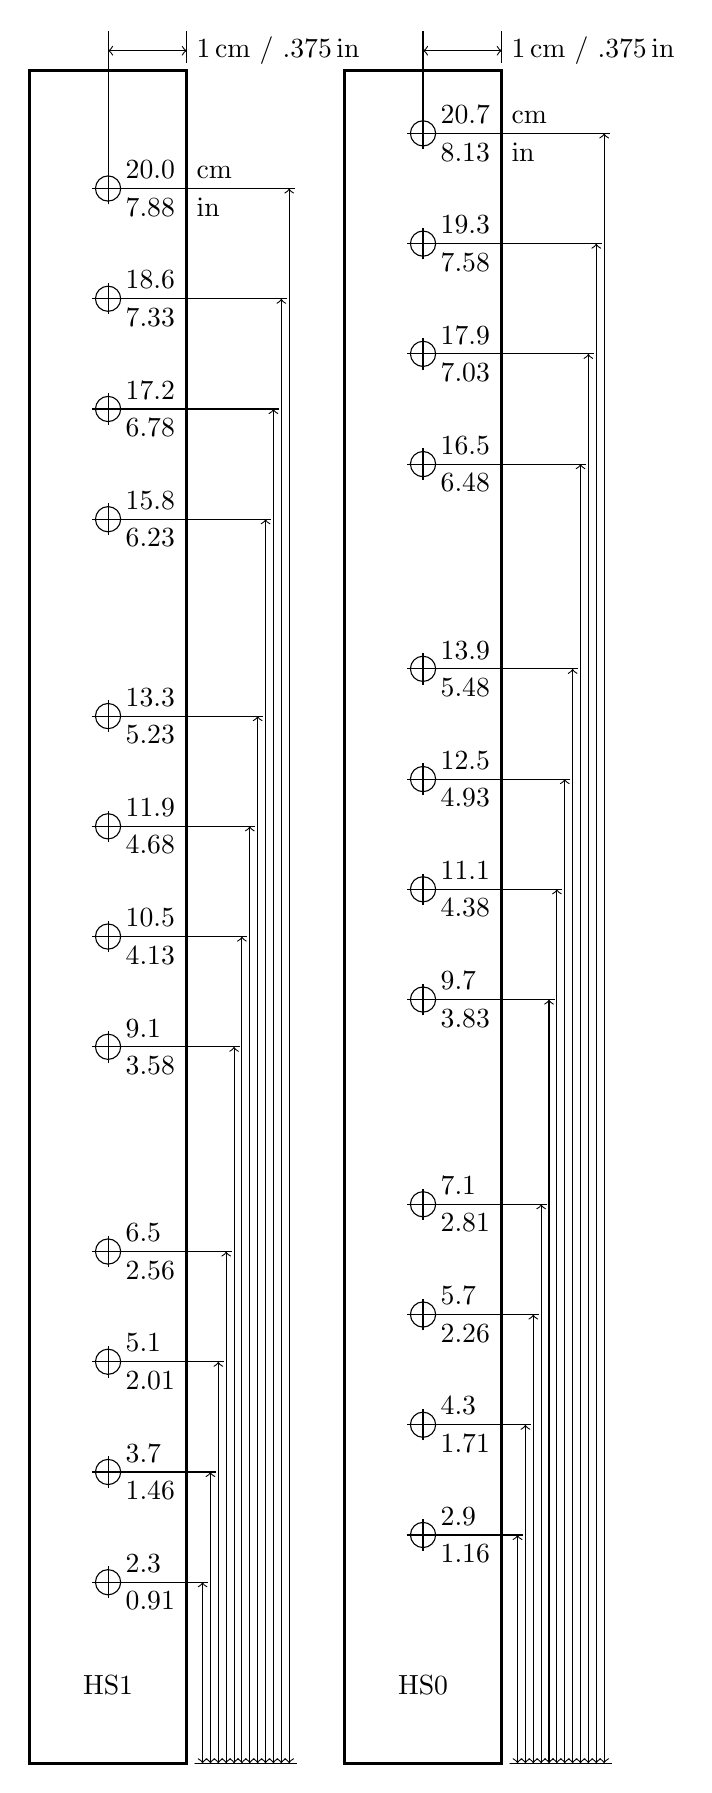
\begin{tikzpicture}
  \draw [very thick] (0,0) -- (0,21.5) -- (2,21.5) -- (2,0) -- cycle;
  \foreach \yy / \y / \z in {0/2.3/0.91, .1/3.7/1.46, .2/5.1/2.01, .3/6.5/2.56, 
		.4/9.1/3.58, .5/10.5/4.13, .6/11.9/4.68, .7/13.3/5.23, 
		.8/15.8/6.23, .9/17.2/6.78, 1.0/18.6/7.33, 1.1/20.0/7.88} {
    \draw (1,\y) circle (0.16);
    \draw (.8,\y) -- (1.2,\y);
    \draw (1,\y-.2) -- (1,\y+.2);
    \draw [<->] (2.2+\yy,0) -- (2.2+\yy,\y);
    \draw (1,\y) -- (2.27+\yy,\y);
    \node [above right] at (1.1,\y) {\y};
    \node [below right] at (1.1,\y) {\z};
    \draw (2.1,0) -- (3.4,0);
  }
  \node [above right] at (2,20) {cm};
  \node [below right] at (2,20) {in};
  \draw (1,20) -- (1,22);
  \draw (2,21.6) -- (2,22);
  \draw [<->] (2,21.75) -- (1, 21.75);
  \node [right] at (2,21.75) {1\,cm / .375\,in};
  \node at (1,1) {HS1};

  \draw [very thick] (4,0) -- (4,21.5) -- (6,21.5) -- (6,0) -- cycle;
  \foreach \yy / \y / \z in {0/2.9/1.16, .1/4.3/1.71, .2/5.7/2.26, .3/7.1/2.81, 
		.4/9.7/3.83, .5/11.1/4.38, .6/12.5/4.93, .7/13.9/5.48, 
		.8/16.5/6.48, .9/17.9/7.03, 1.0/19.3/7.58, 1.1/20.7/8.13} {
    \draw (5,\y) circle (0.16);
    \draw (4.8,\y) -- (5.2,\y);
    \draw (5,\y-.2) -- (5,\y+.2);
    \draw [<->] (6.2+\yy,0) -- (6.2+\yy,\y);
    \draw (5,\y) -- (6.27+\yy,\y);
    \node [above right] at (5.1,\y) {\y};
    \node [below right] at (5.1,\y) {\z};
    \draw (6.1,0) -- (7.4,0);
  }
  \node [above right] at (6,20.7) {cm};
  \node [below right] at (6,20.7) {in};
  \draw (5,20.7) -- (5,22);
  \draw (6,21.6) -- (6,22);
  \draw [<->] (6,21.75) -- (5, 21.75);
  \node [right] at (6,21.75) {1\,cm / .375\,in};
  \node at (5,1) {HS0};
 \end{tikzpicture}
 \caption{Drill Locations for Heat Sinks HS0--HS1\label{fig:hsdrill}}
\end{figure}

\chapter{Assembling the PC Board}\label{ch:assembly}
\LLstart{W}{ITH}{all the parts} and tools at hand as described in the previous chapter, you
are now ready to begin assembly of the Lumos controller PC board.  The order of installation
presented here is intended to make assembly as convenient as possible.  Generally this means
progressing from the shortest to the tallest components, allowing the board to be laid flat
face-down on the work surface while soldering the component leads.

\begin{itemize}
\item[\HandRight] \bfseries{Note:} 
Take care to make good, solid \ix{solder connections} when installing components.
Hold your soldering iron to the part's lead \emph{and} the \ix{annular ring} of the \acronym{PCB}
until both are hot, then apply just enough solder to cover the ring, withdraw the solder, then 
remove the heat.  Good solder connections should be shiny and smooth.

\item[\HandRight] \bfseries{Note:} 
The board layout is quite compact, with many components in a small space.  Take
care when soldering that you don't accidentally heat the wrong component or form solder bridges between
nearby contact points.

\item[\HandRight] \bfseries{Note:} 
We will point out a few places where \acronym{ESD} protection is needed, but
that is intended to call attention to the issue at some key points, not to be a comprehensive list of
\emph{every} case where it is needed.  You are expected to use appropriate handling protocols for all
parts, which includes the use of \acronym{ESD} protection when working with semiconductors (e.g., all
chips, voltage regulators, transistors, etc.).
\end{itemize}


\section{Building the Relay Section}
Refer to Figure~\ref{fig:placement} throughout these instructions to see where the components are 
located on the \acronym{PCB}.  The locations are also labeled on the \acronym{PCB} itself.

\begin{figure}
\centerline{\LLimg{24dc-parts-placement}}
\caption{Lumos Board Parts Placement Diagram\label{fig:placement}}
\end{figure}
\begin{figure}
\centerline{\LLimg{24dc-parts-placement-back}}
\caption{Lumos Board Parts Placement (Reverse Side)\label{fig:placement-back}}
\end{figure}

\begin{enumerate}

\item\label{s:resistor1}
	Install (3) 220\,$\Omega$ \ix{resistors} in positions R6--R8 as marked on the \acronym{PCB}
	and Figure~\ref{fig:placement}.  These have the color bands ``red-red-brown'' 
	marking them.  Push them all the way until flush with the \acronym{PCB}.
\item	solder their leads on the bottom side of the board.  
\item\label{s:resistor2}
	Trim the excess leads with \ix{diagonal cutters}.
\item	Repeat steps \ref{s:resistor1}--\ref{s:resistor2} to 
	install (24) 470\,$\Omega$ \ix{resistors} (``yellow-violet-brown'') at R9--R32.
\item	Repeat steps \ref{s:resistor1}--\ref{s:resistor2}
	to install (24) 10\,K \ix{resistors} (``brown-black-orange'') at R33--R56.
\item	In the same fashion, install and solder (3) 0.33\,$\mu$F \ix{capacitors} into positions marked C0--C2.
\item	Install and solder (3) 0.1\,$\mu$F capacitors into positions C3--C5.
	{\bfseries NOTE: Capacitor C3 is located nearest to C0 on the \acronym{PCB}. On
	board versions through 1.0.8, this is mis-labeled as ``C1.''}
\item	Install (3) 1N4004 \ix{diodes} at D0--D2.  {\bfseries Note: These parts will not function
	if inserted the wrong direction.} Each diode has
	a stripe on one end. This end is inserted into the hole marked by the straight line (cathode)
	drawn on the \acronym{PCB}.  The unmarked end goes into the hole marked by the triangle
	(anode).  Solder into place. 
\item	Install (3) green \acronym{LED}s at D3--D5.  {\bfseries Note: These must be inserted in the 
	correct orientation.} The longer lead (anode) goes into the square hole, while the shorter
	lead (cathode) goes into the round hole.  Solder into place.
\item	Note the location of U0--U5 and R0--R5 (located \emph{inside} the borders of chips U0--U5).
\item	Flip the board over to the bottom (solder) side.  Be sure you still see where R0--R5 are
	located.
\item\label{s:R0s}
	Install (1) 680\,$\Omega$ \ix{resistor network} \emph{on the bottom (solder) side} of the board at
	R0 (the row of six holes \emph{inside} U0).  {\bfseries Note the correct position of R0.} The
	square hole on the \acronym{PCB} marks where pin~1 of R0 should be inserted.  Pin~1 is marked
	with a dot on R0 itself. See Figure~\ref{fig:placement-back}.
	\marginpar{\LLimg[width=1in]{resistor-network}}
\item	Holding R0 in place, carefully flip the board over.
\item\label{s:R0e}
	Keeping R0 straight, solder into place (soldering on the component side of the \acronym{PCB}).
\item\label{s:R1}
	Repeat steps \ref{s:R0s}--\ref{s:R0e} to install R1 on the bottom side of the \acronym{PCB},
	inside U1's space.  {\bfseries Caution:} Pin~1 of R1 still goes in the square hole, but 
	beware---this location is the mirror image of where it was for R0.  In other words, pin~1
	of R0 and R1 are next to one another.
\item	Repeat steps \ref{s:R0s}--\ref{s:R1} to install (4) more resistor networks at R2--R5.
\item	Flip the board back over to the component side.  {\bfseries Caution:} From this point 
	forward, don't forget those resistors are on the other side of the board.  If you press down
	on the board (e.g., when installing chips into sockets), you will bend the resistors and may
	break them.
\item	Install (6) 16-pin \acronym{DIP} sockets XU0--XU5 in positions marked U0--U5.  
	Note that they need to fit easily
	over the soldered leads from R0--R5.  If they don't, select a different style of socket or
	carefully trim down the resistor leads.
\item	Solder sockets XU0--XU5.
\item	Install (3) 4-position \ix{jumper block} headers at J6--J8.  Solder.
\item	Install (3) LM78L05 voltage regulators at U6--U8.  
	{\bfseries These parts will not function unless oriented correctly.}  Note the flat side on
	the component case.  This aligns with the flat side drawn on the circuit board.
	Apply \ix{heat protection} while soldering in
	place, and/or limit soldering time to 4 seconds or less.  Use \acronym{ESD} protection.
\item	Install (3) \ix{fuse holders} at F0--F2.  Due to the wide \acronym{PCB} traces here, this may require
	extra soldering time, but be careful not to overheat the parts.  The same will be true for
	steps \ref{s:tb1}--\ref{s:tb2}.
\item\label{s:tb1}
	Install (3) 10-position terminal blocks at J0--J2.  
\item\label{s:tb2}
	Install (3) 2-position terminal blocks at J3--J5.
\item\label{s:MOSFET1}
	Using \acronym{ESD} protection, lay out (12) \acronym{MOSFET}s on your workbench.
\item	Prepare each \acronym{MOSFET} by bending the middle lead 90$^\circ$ up toward the front
	of the transistor body, then move your pliers down the lead another 0.1$''$ and bend it
	90$^\circ$
	back again, parallel to the other pins again.  It should now look like the photo
	in Figure~\ref{fig:mosfet} and should fit
	easily into the holes at Q0 on the \acronym{PCB}.
\begin{figure}
	\centerline{\LLimg[height=3in]{mosfet-side} \LLimg[height=3in]{mosfet-board}}
	\caption{Bending the Pins of the M\mc{OSFET}s\label{fig:mosfet}}
\end{figure}
\item	Apply a \emph{small} dab of \ix{heat sink} grease on the back side of the transistor.
\item\label{s:MOSFET2}
	Bolt the transistor onto heat sink HS0, with the washer and nut on the transistor side,
	making sure to smear the heat sink grease in a thin layer between the heat sink and
	the transistor.  Make the part snug but not over-tight, and approximately 90$^\circ$
	perpendicular to the heat sink bar.
\item	Repeat steps \ref{s:MOSFET1}--\ref{s:MOSFET2} for the remaining transistors until you have
	a row of 12 bolted to the heat sink.
\item	Position the heat sink over all the even-numbered positions Q0--Q22 on the \acronym{PCB},
	carefully adjusting the position of each part until all 36 pins slide into their holes.
	Push the entire set very carefully into place until all transistors are seated as far as they
	will go.  {\bfseries Note:} Due to irregularities in hole placement on the heat sink, it's
	possible the transistors won't all be \emph{perfectly} straight, but they should be as
	close as possible.  You may need to loosen the bolts slightly to position the 
	transistors, then tighten again when they are in place.
\item	Using appropriate heat protection and/or limiting soldering time to 4 seconds or less per
	pin, solder the leads of the 12 transistors into place.  
\item\label{s:MOSFET3}
	Trim the excess leads.
\item	Repeat steps \ref{s:MOSFET1}--\ref{s:MOSFET3} for another 12 transistors, except:
%with the following changes:
	\begin{itemize}
		\item	Bolt them to the heat sink HS1 with the nut and washer on the side opposite the
			transistor.
		\item	Insert them into the odd-numbered locations Q1--Q23.
		\item	When finished, there should be a slight air gap between the two rows of
			transistors.
	\end{itemize}
\item	Insert (6) K847PH \ix{opto-isolator chips} into their sockets at U0--U5.  {\bfseries Note:} pin~1
	of each chip is marked with a small triangle on the \acronym{PCB} and a square hole.
\item	Insert (3) 10\,A \ix{fuses} into the fuse holders.
\end{enumerate}

This completes the assembly of the relay portion of the Lumos board, common to all configurations.

\bigskip

\noindent {\bfseries Skip} ahead to Chapter~\ref{ch:cpu} if you are making a normal (``intelligent'') Lumos controller.

\bigskip

\noindent{\bfseries Continue} to the rest of this chapter if you are making a ``dumb'' relay-only board instead.

\section{Making a Relay-Only Lumos Board}
If you only want relays with no intelligent logic on-board, perform the following additional
steps to allow the board to accept external control signals from another circuit.  {\bfseries Do not
do the following if you will be adding the intelligent on-board controller (``\acronym{CPU}'' option)!}
\begin{enumerate}
\item	
	Install a 26-pin male header at J14 (inside the boundaries of the 40-pin chip U9, which will
	not be installed on this board).  Note the location of pin 1, as marked by a triangle on the
	\acronym{PCB}.  Align this with pin 1 on the header part, usually marked by a triangle or arrow
	engraved on the plastic.  There is also usually a key in the center of the side where pin~1
	is located.  Solder into place.
\item	
	Install a 220\,$\Omega$ resistor (``red-red-brown'') 
	into the bottom two holes (this is the square hole and the
	immediately adjacent round hole) of R60 (see Figure~\ref{fig:R60-singleton}).  Solder into place.
\item	
	Install a green \acronym{LED} at D8.  As before, note that {\bfseries this must be inserted
	in the correct orientation.} The longer lead (anode) goes into the square hole, while the shorter
	lead (cathode) goes into the round hole.  Solder into place.
\end{enumerate}

Your relay-only board is now complete and ready to plug into the controlling circuit which will
be driving it.  For details on how to plug it in, see the connector pinout diagrams in the appendices,
and the theory of operation section of \emph{Using Lumos SSR Controllers} as it applies to the way
signals are sent to the relays, since your controlling circuit will need to do this directly via
its connection at J14.

If you also want to install the logic output option, skip to Chapter~\ref{ch:logic-out} now.  Otherwise,
you are finished.  {\bfseries No other options may be installed on this board.} They all require
an intelligent controller on-board.

\bigskip

\noindent{\bfseries Stop.}

\chapter{Assembling the CPU Option}\label{ch:cpu}
\LLstart{W}{ITH}{the basic relay circuits} in place, the next step in Lumos controller construction
is to add the control logic.  You will be adding the microcontroller ``brain'' of the Lumos board
which turns the relays on and off according to the commands and programs it receives.

Follow these steps to add the \acronym{CPU} to your Lumos board:
\begin{enumerate}
\item	Install a 33\,K resistor (``orange-orange-orange'') at position R57.  Solder into place.
\item	Install a 330\,$\Omega$ resistor (``orange-orange-brown'') at position R61.  Solder into place.
\item	Install a 40-pin \acronym{DIP} socket at U9. Solder into place.

\item	Install (2) 30\,pF capacitors at positions C6 and C7. Solder into place.
\item	Install a 0.1\,$\mu$F (100\,nF) capacitor at C8 and C12.  Solder into place.
\item	Install a 0.01\,$\mu$F (10\,nF) capacitor at C9. Solder into place.
\item	Install a 0.33\,$\mu$F (330\,nF) capacitor at C11.  Solder into place.
\item	Install a 220\,$\Omega\times$5 resistor network at R60.  Ensure the dot on the resistor package
	(pin~1) goes into the square hole (marked by a triangle).  Solder into place.
\item	Install a 1N4004 diode at D6.  {\bfseries This part will not function if not oriented
	correctly.} Be sure the stripe printed on the diode is on the side inserted into the
	square hole, and marked with a straignt line, while the other, unmarked lead goes in the
	round hole marked with a large triangle.  Solder into place.
\item\label{s:header}
	Install a five-pin header at J11.  Keep the pins straight and perpendicular to the board
	while soldering into place.
\item	Repeat Step~\ref{s:header} for the four-pin header at J17.
\item	Install a two-position terminal block at J10.  Solder into place.
\item	{\bfseries Using proper static protection,} prepare U11 for insertion by bending its
	leads 90$^\circ$ back toward the back of the part, with the center pin about 0.1$''$ longer
	before the bend.  Bend the pins to the right locations so that the pins easily
	slip into the holes at U11 with the large tab mounting hole aligned with the corresponding hole in
	the \acronym{PCB}.
\item	Place a TO-220 heat sink on the board at U11, with its hole aligned with the hole in the
	\acronym{PCB} at U11.
\item	Place a small dab of thermal grease on the back of U11, then slip its pins through the holes
	at U11 on the board, laying it down on the heat sink.  Secure U11 by installing a \#6
	bolt through U11, through the heat sink, all the way through the \acronym{PCB}, terminated
	by a nut on the opposite side.  Tighten but don't over-tighten.  Solder the three leads
	into place.
\item	Install a 10\,MHz crystal at X0.  Solder into place.


\item\label{s:resetbtn}
	Install a red push-button at S0 (``reset'').  {\bfseries This part will not function if
	not oriented correctly.} Be sure to line up  the indentations on one side of the button
	with the silk screened image.  The button should be oriented so that the top two pins
	short to the bottom to pins when the button is pressed.  Ensure the button is straight
	and solder into place.
\item
	Repeat step~\ref{s:resetbtn} to install a green push-button at S1.
\item
	Install the pre-programmed \mc{PIC}18\mc{F}4685 microcontroller chip into its socket at U9.
	{\bfseries This part will not function if not oriented correctly.}  Pin~1 is marked by
	the indentation on the chip body outline on the board.  Pin~1 is also marked by a triangle.
\end{enumerate}

The following instructions depend on which other options you selected for your board.
Perform each in the order shown here.

\begin{description}
\item[IF] 
	you will be installing any sensor inputs 
	{\bfseries OR} you wish to attach front-panel \acronym{LED}s for diagnostic output rather than
	the on-board \acronym{LED}s,
\item[THEN] do the following:
	\begin{enumerate}
	\item	Review all of Chapter~\ref{ch:sensor-in} to determine which, if any, \acronym{LED}s you
		will install on the board, and which will be omitted.
	\item	Install a 10\,K$\times$5 resistor network at R59.  Ensure the dot on the resistor package
		(pin~1) goes into the square hole (marked by a triangle).  Solder into place.
	\item	Install a 5-position terminal block at J16 (this will also occupy J9).  Solder into place.
	\item\label{s:powerLED}
		Install a green \acronym{LED} at D8. {\bfseries This part will not function if not
		correctly oriented.} Insert the longer lead (anode) into the square hole on the
		board. The shorter lead (cathode) goes into the round hole. Solder into place.
	\item	Repeat Step~\ref{s:powerLED} to install the \acronym{LED}s you didn't decide 
		to exchange for sensor inputs (if any) into positions D7 (red), D9 (yellow),
		D10 (green), and D11 (yellow).  Solder into place.  {\bfseries Omit this step}
		if you are moving the \acronym{LED}s to the front panel.
	\end{enumerate}
\item[OTHERWISE] do the following:
	\begin{enumerate}
	\item	Install a 10\,K resistor at R58.  Note that it goes into the square hole (marked with a
		triangle on the board) and the second hole to the left of it (there will be one empty hole
		under the resistor, between the leads).  See Figure~\ref{fig:R58} for details.  Solder
		into place.
	\item	Install a 2-position terminal block at J9.  This will go into the two right-most holes
		(the ones marked with triangles).  Solder into place.
	\item\label{s:diagLED}
		Install a red \acronym{LED} at D7.  {\bfseries This part will not function if not
		correctly oriented.} Insert the longer lead (anode) into the square hole on the	
		board. The shorter lead (cathode) goes into the round hole.  Solder into place.
	\item   Repeat Step~\ref{s:diagLED} to install (2) green \acronym{LED}s at D8 and D10.
	\item   Repeat Step~\ref{s:diagLED} to install (2) yellow \acronym{LED}s at D9 and D11.
	\end{enumerate}
\end{description}

This completes the installation of the \acronym{CPU} option.  

\bigskip

\noindent{\bfseries Continue} to the following sections
to install the other options you selected.

\chapter{Assembling the Communications Options}\label{ch:comms}
\LLstart{A}{N}{Intelligent controller board} needs some way to receive commands from the outside
world.  Three different options are available: RS-485 full duplex, RS-485 half duplex, and RS-232
(standard serial).  (If you will be using the Lumos controller with \acronym{DMX512}, build the
board with one of the RS-485 options.  The \acronym{DMX512} mode of operations will only 
accept commands and never transmit data back, so it will not take advantage
of the full duplex capability, but you may wish to have full duplex for Lumos mode operations
or for programming and configuring the board.

\bigskip

\noindent{\bfseries Skip} to the section below which describes the communication option
you have selected.  You must do exactly {\bfseries one} of these.

\section{RS-485 Full Duplex / DMX512}
Perform the following steps to add {\bfseries full-duplex} RS-485 capability:
\begin{enumerate}
\item	Install a 10\,K resistor (``brown-black-orange'') at R62.  Solder into place.
\item\label{s:u13pin1}
	Install a 14-pin \acronym{DIP} socket at U13.  Note the position of pin~1 (indicated
	by a square pad and silk-screened triangle).  If your socket also indicates pin~1, align
	it to match the \acronym{PCB}. Solder into place.
\item	Install a 0.01\,$\mu$F (10\,nF) capacitor at C10. Solder into place.
\item	Install a fuse holder at F3.  Solder into place.  This is optional (you could solder a fuse
	directly onto the board, but the holder is recommended.  It makes it far easier to replace
	the fuse if it should ever blow.
\item	Install an 800\,mA fuse at F3.  Clip the leads to the appropriate length so it will rest
	all the way down into the socket.
\item	Install (2) 8p8c modular jacks at J12 and J13, noting the position of pin~1 as indicated by
	square pads and silk-screened triangles.  Solder into place.
\item	If the other devices you will plug together share a common notion of ``ground'' a wire jumper
	may be installed in place of R63.  Otherwise, if you need to protect against ground loops,
	install a 100\,$\Omega$ resistor (``brown-black-brown'') at R63. Solder into place.
\item	Install a MAX489 driver/receiver chip into its socket at U13, noting the marked location
	of pin~1 (see Step~\ref{s:u13pin1}).  Press carefully down into place.
\end{enumerate}

\bigskip\noindent{\bfseries Skip} to the section on RS-485 terminators below.

\section{RS-485 Half Duplex}
Perform the following steps to add {\bfseries half-duplex} RS-485 capability:
\begin{enumerate}
\item	Install a 10\,K resistor (``brown-black-orange'') at R62.  Solder into place.
\item\label{s:u10pin1}
	Install an 8-pin \acronym{DIP} socket at U10.  Note the position of pin~1 (indicated
	by a square pad and silk-screened triangle).  If your socket also indicates pin~1, align
	it to match the \acronym{PCB}. Solder into place.
\item	Install a 0.01\,$\mu$F (10\,nF) capacitor at C10. Solder into place.
\item	Install a fuse holder at F3.  Solder into place.  This is optional (you could solder a fuse
	directly onto the board), but the holder is recommended.  It makes it far easier to replace
	the fuse if it should ever blow.
\item	Install an 800\,mA fuse at F3.  Clip the leads to the appropriate length so it will rest
	all the way down into the socket.
\item	Install (2) 8p8c modular jacks at J12 and J13, noting the position of pin~1 as indicated by
	square pads and silk-screened triangles.  Solder into place.
\item	If the other devices you will plug together share a common notion of ``ground'' a wire jumper
	may be installed in place of R63.  Otherwise, if you need to protect against ground loops,
	install a 100\,$\Omega$ resistor (``brown-black-brown'') at R63. Solder into place.
\item	Install an SN75176 driver/receiver chip into its socket at U10, noting the marked location
	of pin~1 (see Step~\ref{s:u10pin1}).  Press carefully down into place.
\end{enumerate}

\bigskip\noindent{\bfseries Continue} to the section on RS-485 terminators below.

\section{RS-485 Terminator Construction}\label{sec:terminator}
Each end of an RS-485 communications line must be terminated, or it won't work.
% (in fact, without termination
%it might not even work \emph{at all}).  
The schematic for this is on page~\pageref{sch:terminator} in the 
appendices.  To build one yourself, you'll need:
\begin{itemize}
\item	(2) 120\,$\Omega$ resistors.
\item	Lumos RS-485 terminator \acronym{PCB}.
\item	A short length of \acronym{CAT5} cable.
\item	An 8p8c male modular plug with detachable boot.
\item	A modular plug crimping tool.
\end{itemize}
Perform the following steps:
\begin{enumerate}
\item	Cut the following lengths of \acronym{CAT5} cable:
	\begin{enumerate}
	\item	(2) 2$''$ (5\,cm) lengths of orange wire.
	\item	(2) 2$''$ (5\,cm) lengths of blue wire.
	\item	(1) 2$''$ (5\,cm) length of green wire.
	\end{enumerate}
\item	Strip \sfrac{1}{4}$''$ (4\,mm) of insulation from \emph{one} end of the orange and blue
	wires.
\item	Refer to the diagram in Figure~\ref{fig:terminator-pcb}.  Solder an orange wire to 
	hole \#2.
\item	Solder another orange wire to hole \#4.
\item	Solder a blue wire to hole \#6.
\item	Solder another blue wire to hole \#8.
\item	Install a 120\,$\Omega$ resistor (``brown-red-brown'') between holes \#1 and \#3.  Solder
	into place.
\item	Install a 120\,$\Omega$ resistor (``brown-red-brown'') between holes \#5 and \#7.  Solder
	into place.
\item 	The board should now look like Figure~\ref{fig:terminator-pcb-wired}.
\item	Arrange all the wires in a row so they are straight and parallel, with the colors in
	the following order:
	\begin{itemize}
	\item	orange
	\item	orange
	\item	green
	\item	blue
	\item	blue
	\item	green
	\end{itemize}
	Note that there is only one green wire.  One end will be at position 3 in the set of wires,
	the wire will loop around and the other end appears at position 6.  Allow enough of the green
	wire to loop around the board without interfering with it, leaving the excess wire with the
	bundle of other wires you're arranging.
\item	Carefully, so as not to disturb the order of the wires, trim the excess wire so the length from the
	end of the \acronym{PCB} to the end of the wires is about 1$''$ or 25\,mm.  Be sure to make the 
	cut so you leave a clean, straight end to the bundle of wires, so they all end at the same
	place.
\item	Carefully, so as not to disturb the order of the wires, insert them into an 8p8c male plug
	shell, with the first orange wire at pin~1 of the plug and the last green wire at pin~6.
	Note that pins~7 and~8 will have no connection.  Push the wires all the way to the end so they
	are snug against the end of the plug.
\item	While applying gentle but firm pressure to hold the wires all the way in position, insert the
	plug into a modular jack crimping tool. Crimp the plug onto the wires.
\item	Cover the end with a plastic boot or other suitable protection.
\end{enumerate}

This completes the assembly of an RS-485 full-duplex terminator with cable-check pins, suitable
for use with full-duplex or half-duplex Lumos boards.  It may nor may not be compatible with other
RS-485 gear.

\bigskip\noindent{\bfseries Skip} to the next chapter to install more options, if desired.

\section{RS-232}
If you will be using a standard RS-232 serial port to communicate with your Lumos board,
perform the following steps to add this capability to the basic \acronym{CPU} circuit:
\begin{enumerate}
\item\label{s:u12pin1}
	Install a 20-pin \acronym{DIP} socket at U12.  Note the position of pin~1 (indicated
	by a square pad and silk-screened triangle).  If your socket also indicates pin~1, align
	it to match the \acronym{PCB}. Solder into place.
\item	Install a 1\,$\mu$F electrolytic capacitor at C13. {\bfseries This component will not
	function unless installed in the correct orientation.}  Note the positive lead is indicated
	on the \acronym{PCB} with a square hole and a silk-screened ``+'' mark; however, it is typical
	for electrolytic capacitors to mark the \emph{negative} lead in some way (usually with an arrow
	and ``$-$'' sign printed on the package).  Solder into place.
\item	Install a female DE-9 (9-pin D-subminiature serial) jack at J15, 
	noting the position of pin~1 as indicated by a square pad.  Solder into place.
\item	Install a MAX232A driver/receiver chip into its socket at U12, noting the marked location
	of pin~1 (see Step~\ref{s:u12pin1}).  Press carefully down into place.
\end{enumerate}

This completes the installation of the RS-232 serial option.

\bigskip\noindent{\bfseries Continue} to the next chapter to install more options, if desired.

\chapter{Assembling the Sensor Input Option}\label{ch:sensor-in}
\LLstart{L}{UMOS}{boards support the option} of attaching up to four simple \acronym{TTL}-level
logic inputs.  The host PC can query the Lumos board to find out the current state of these
inputs.  The Lumos board may also be programmed to react on its own to a change in the input states.

These inputs may come from sensors (e.g., light sensors or motion sensors) which produce a compatible
output signal.  They may even come from the logic outputs of another Lumos board.

The trade-off here, however, is that the signal lines used by the sensors are also used to drive
the diagnostic \acronym{LED}s.  Any given line may only be a sensor input \emph{or} an \acronym{LED}
output at any given point in time, but never both.

It is generally recommended that you decide in advance how many sensor inputs you will need, then
look at the table of diagnostic codes in \emph{Using Lumos SSR Controllers} to determine which
specific \acronym{LED}s you're willing to live without.  Those \acronym{LED}s should then be omitted
from the construction of the board's \acronym{CPU} option, so they won't interfere with the
inputs coming in on the same pins of the microcontroller.

The correspondence of \acronym{LED}s to inputs is shown in Figure~\ref{tbl:led-inputs}.
\begin{figure}[htb]
 \begin{center}
  \begin{tabular}{|c|ll|}\hline
    \bfseries Sensor & \multicolumn{2}{c|}{\bfseries Diagnostic \acronym{LED}} \\\hline\hline
    {\LARGE\strut}$\overline{\hbox{A}}$ & D7  & ``Status'' (red) \\\hline
    {\LARGE\strut}$\overline{\hbox{B}}$ & D10 & ``Status'' (green) \\\hline
    {\LARGE\strut}$\overline{\hbox{C}}$ & D9  & ``Activity'' (yellow) \\\hline
    {\LARGE\strut}$\overline{\hbox{D}}$ & D11 & ``Status'' (yellow) \\\hline
  \end{tabular}
 \end{center}
 \caption{\label{tbl:led-inputs}Mapping of Diagnostic \acronym{LED}s to Input Sensors}
\end{figure}

These are named as active-low inputs (i.e., ``$\overline{\hbox{A}}$'' instead of ``A'') because that
is a common model and is compatible with the Lumos logic output lines which are active-low signals.
As such, the Lumos board includes a 10\,K pull-up resistor connected to each of the input lines
so they will default high unless explicitly pulled low by the input.  It may be actively driven low
or high by the sensor.  The Lumos board may, however, be programmed to respond to the inputs as if
they were active-high or active-low.  There shouldn't therefore be a need to invert an active-high
input for use with a Lumos board.

\section{What If I Want to Keep All My LEDs?}
A natural question to ask here is, ``Can I keep the \acronym{LED}s installed \emph{and} 
have sensor inputs, deciding at different times to configure the Lumos board to treat them
as inputs or \acronym{LED}s as needed at that moment?''

The answer is ``maybe.''  It depends on what you plug into the sensor inputs and how much
current it can supply, since it would have to power the \acronym{LED}s too.  

Normally, the sensor inputs have the effective circuit shown in Figure~\ref{fig:input-normal}.
However, if the \acronym{LED} is physically present on the board at the same time, the effective
circuit becomes the one shown in Figure~\ref{fig:input-led}.  Consider whether your input source
can tolerate that circuit configuration before proceeding.  If it can't, you need to remove the
\acronym{LED}(s) corresponding to the input lines you'll use.
\begin{figure}[htb]
  \begin{circuitikz}
    \node [left] at (0,0) {Sensor Input};
    \draw (0,0) -- (1,0) -- (.8,.2) -- (1,0) -- (.8,-.2);
    \draw (1,.2) -- (1.2,0) -- (1,-.2);
    \draw (1.2,0) -- (6,0);
    \draw [thick] (8,3) -- (6,3) -- (6,-1) -- (8,-1);
    \node [right] at (6,2) {Microcontroller};
    \node [right] at (6,0) {I/O port};
    \node [below] at (1,-.2) {J16};
    \draw (2,1) to [R, l={10\,K}] (2,3);
    \draw (2,1) -- (2,0);
    \draw (1.6,3) -- (2.4,3);
    \node [above] at (2,3) {+5\,V};
    \draw [fill] (2,0) circle (.1);
  \end{circuitikz}
  \caption{\label{fig:input-normal}Sensor Input Circuit}
\end{figure}
\begin{figure}[htb]
  \begin{circuitikz}
    \node [left] at (0,0) {Sensor Input};
    \draw (0,0) -- (1,0) -- (.8,.2) -- (1,0) -- (.8,-.2);
    \draw (1,.2) -- (1.2,0) -- (1,-.2);
    \draw (1.2,0) -- (6,0);
    \draw [thick] (8,3) -- (6,3) -- (6,-1) -- (8,-1);
    \node [right] at (6,2) {Microcontroller};
    \node [right] at (6,0) {I/O port};
    \node [below] at (1,-.2) {J16};
    \draw (2,1) to [R, l={10\,K}] (2,3);
    \draw (2,1) -- (2,0);
    \draw (1.6,3) -- (2.4,3);
    \node [above] at (2,3) {+5\,V};
    \draw [fill] (2,0) circle (.1);
    \draw [fill] (3,0) circle (.1);
    \draw (3,0) to [full led] (3,-2);
    \draw (3,-2) to [R, l={220\,$\Omega$}] (3,-4) node[ground] {};
  \end{circuitikz}
  \caption{\label{fig:input-led}Sensor Input Circuit with \acronym{LED} Present}
\end{figure}
    

\section{Installing the Option Hardware}

To install this option, do the following:
\begin{enumerate}
\item	Install a 10\,K$\times$5 resistor network at R59.  {\bfseries This component will not
	function if not oriented correctly.} Pin~1 (the common pin) is marked with a dot on the 
	resistor itself.  This goes into the hole marked with a square pad and silk-screened 
	triangle.  Note that R59 takes the place of R58 on the Lumos board.  If you're adding this
	option to an existing Lumos board which was built without this option originally, you 
	will need to remove R58 first.  Keeping the pins straight, solder R59 into place.
\item	Install a five-position terminal strip at J16.  Note that this takes the place of J9.
	If you're adding this option to an existing Lumos board which was originally completed
	without inputs, you will need to remove J9 first.  Solder J16 into place.
\end{enumerate}

\begin{description}
\item[\HandRight\ Note:] Before any inputs will be recognized, the Lumos board must be configured
in software to change those specific lines from \acronym{LED} outputs to logic inputs.  See
\emph{Using Lumos SSR Controllers} for programming and configuration details.
{\bfseries Never attach sensors to the terminal block at any time the Lumos board is software-configured
to drive those lines as \acronym{LED}s.  
\item[\HandRight\ Note:] Always configure those as inputs before attaching the
sensor hardware.} Otherwise, the Lumos board will try to drive those \acronym{LED}s, which the
sensors may not tolerate well. If the sensor is also driving the line at the same time, you may
short out those input pins on the microcontroller, causing damage.
\end{description}

This completes the construction of the sensor input option.

\bigskip\noindent{\bfseries Continue} to the next chapter to add more options if desired.

\chapter{Assembling the Logic Output Option}\label{ch:logic-out}
\LLstart{I}{F}{you need to control} 1--4 \acronym{TTL}-level outputs from the Lumos board,
this can be accomplished by adding the Logic Output Option to the basic unit.  This can be
added to any Lumos board, even ``dumb'' relay-only boards.  

To provide this option, simply install a five-position terminal strip at J18 and solder it
into place.

Having done that, the raw logic-level outputs for channels 0--3 from the controlling 
circuit (either external or the on-board microcontroller) are present on J18, along with a ground
reference.

\begin{description}
\item[\HandRight\ N.B.:] These outputs are straight from the logic circuitry which drives the
Lumos relays.  They are \emph{not} isolated like all the other power outputs are.  Care should
be exercised when attaching these outputs to other devices.
\end{description}

\bigskip\noindent{\bfseries Continue} to the next chapter to install more options, if desired.

\chapter{Using a Front Panel}\label{ch:fp}
\LLstart{M}{any}{controllers are installed} into a weather-resistant enclosure which allows access
to the circuit board to make connections and to access the buttons and \acronym{LED}s.  If the Lumos
board will be installed in a more closed box it would be desirable to bring the \acronym{LED}s, buttons,
and other connections to panel-mount components.

For power connections, there are a variety of panel-mount connectors which may be employed and wired
back to the terminal strips on the Lumos board.  Select those which work for your application.
Since the power connections need jumpers to select the input voltage, you may need to bring those
selectors out to a front or back panel as well.  You can easily connect a \acronym{DPDT} switch
to a 4-position connector which attaches to the jumper blocks.  The wiring arrangement for this 
is shown on page~\pageref{sec:voltagesw} in the appendices.

Similarly, network connections may be brought to the outside of the box by installing modular jacks
on the outside, wiring them back to J12 and J13 or J15. 

If external \acronym{LED}s are needed, the easiest approach is to install a terminal strip at J16.
The terminals A--D on that terminal carry the same signals that run the on-board \acronym{LED}s.
See the table in Figure~\ref{tbl:input-leds} to find which terminal carries which \acronym{LED} power.
To avoid overloading the microcontroller's I/O port power capacity, it would be better to remove the
on-board \acronym{LED}s in the cluster D7, D9, D10, and D11 if external \acronym{LED}s will be used
in this manner.  Note that the external \acronym{LED}s require appropriate current-limiting resistors
installed for them.  This is not provided at J16.

The Option and Reset buttons can be external buttons which are wired to a 5-pin connector 
plugged in to J11.  An example front panel circuit is shown in Figure~\ref{sch:fpex}.

%
%       J11-5 J11-3    J16C J16B J16D J16-A
%        |     |         |   |    |    |
%        o     o         A   G    Y    R
%         | O   | R
%        o     o         R
%        |     |         |
%  J11-2-*-----*---------*---*---_*----*
%
% SMART PHONE RECHECK
% intel free press
% CRK togo mobile
% visual ranking app -- monday
%

\begin{figure}
 \begin{circuitikz}
  \node [left] at (-.1,0) {J11-2};
  \draw [fill] (.5,0) circle (.1);
  \draw (0,0) -- +(-.2,.2) -- (0,0) -- +(-.2,-.2);
  \draw (.5,0) to [cspst, l={Option}, label/align=rotate] (.5,4) -- +(-.2,.2) -- +(0,0) -- +(.2,.2);
  \node [above] at (.5,4.2) {J11-5};
  \draw (1.5,0) to [cspst, l={Reset}, label/align=rotate] (1.5,4) -- +(-.2,.2) -- +(0,0) -- +(.2,.2);
  \node [above] at (1.5,4.2) {J11-3};
  \draw [fill] (1.5,0) circle (.1);
  \foreach \color/\x/\name/\t in {yellow/3/Activity/C, green/4.5/Status (G)/B, yellow/6/Status (Y)/D, red/7.5/Status (R)/A} {
	  \draw [color=\color] (\x,4) to [full led] (\x,2);
	  \draw (\x,0) to [R] (\x,2);
	  \draw (\x,4) to [empty led, l={\name}, label/align=rotate] (\x,2);
	  \draw (\x,4) -- ++(0,.2) -- +(-.2,-.2) -- +(0,0) -- +(.2,-.2);
	  \node [above] at (\x,4.2) {J16-\t};
  }
  \foreach \x in {3, 4.5, 6} {
	  \draw [fill] (\x,0) circle (.1);
  }
  \draw (0,0) -- (7.5,0);
 \end{circuitikz}
 \caption{\label{sch:fpex}Example of a Front Panel Circuit for a Lumos Board}
\end{figure}

\chapter{Going On From Here}\label{ch:goingon}
\LLstart{N}{OW}{that your Lumos controller} board is assembled, go on to read the manual
\emph{Installing the Lumos 24-Channel DC Controller} for help in setting up your controller
for use (including cabling and connector pinout information), and
\emph{Using Lumos SSR Controllers} to learn how to control and program it using software.

\backmatter
\appendix

\chapter{Errata}
On \acronym{PCB} version 1.0.8, one of the parts is mis-labeled on the white silk-screened legend.
There are two capacitors labeled ``C1.''  The true C1 is a 0.33\,$\mu$F capacitor next to C4 near the
center of the \acronym{PCB}.  The 0.1\,$\mu$F capacitor next to C0 should have been marked ``C3.''

\input pinouts

\chapter{Schematics}
The following pages contain the schematic diagrams for all the various options that can comprise
a Lumos 24-channel DC controller.

\begin{figure}
\centerfloat{\LLimg[height=\textheight]{24ssr-dc-relays}}
\end{figure}
\begin{figure}
\centerfloat{\LLimg[height=\textheight]{24ssr-dc-controller}}
\end{figure}
\begin{figure}
\centerfloat{\LLimg[height=\textheight]{24ssr-dc-controller-options}}
\end{figure}
\begin{figure}
\centerfloat{\LLimg[height=\textheight]{24ssr-dc-panel}}
\end{figure}

\chapter{Glossary}\label{ch:glossary}
\begin{description}
	\item[Active High:]
		A logic signal which is considered ``on'' when the signal is ``high'' (binary 1 or +5\,V),
		and ``off'' when the signal is ``low'' (binary 0 or 0\,V).  Lumos relay circuits are 
		triggered with active-low signals.
	\item[Active Low:]
		A logic signal which is considered ``on'' and ``off'' at the opposite signal levels
		to an ``active high'' signal (q.v.).
	\item[Annular Ring:]
		The exposed ring of metal around a hole in a \acronym{PCB} where a component is to be 
		mounted.  The solder will flow across the component lead and onto the annular ring.
%	\item[Daisy Chain:]
%		The arrangement of wiring a number of devices together by connecting the first to the second,
%		then adding another connection from the second to the third, and so forth.  The network
%		connection diagram in Figure~\ref{fig:net} shows an example of a daisy chain.
	\item[\acronym{DIP} (Dual In-line Package):]
		The style of chip where the pins are laid out in two parallel rows.
	\item[\acronym{DIY}:] ``Do-It-Yourself.''
	\item[Duplex:]
		a feature of a serial line.  On a full-duplex connection, separate data wires are present
		to carry data in both directions, so one device can send and receive data at the same time.
		On a half-duplex connection, only a single set of data wires is present, so devices must
		take turns transmitting over them.
	\item[\acronym{ESD} (Electro-Static Discharge):]
		static electricity which builds on your skin and is then discharged into sensitive
		components when you touch them.  Invisible to the eye, this can punch microscopic holes
		in the inside of the components, severely damaging them.
	\item[Heat Protection:]
		A temporary heat sink applied to a component when soldering that component onto
		the \acronym{PCB}.  Typically used for heat-sens\-i\-tive components such as transistors
		and integrated circuit chips.
	\item[Jumper Block:]
		A series of pins mounted to the \acronym{PCB}.  Different options are configured for the
		circuit by placing a jumper over certain pairs of pins, shorting them together.
	\item[\acronym{LED} (Light Emitting Diode):]
		A special kind of diode which emits light when current passes from its anode to its cathode.
	\item[\acronym{MOSFET}:]
		The type of transistor which forms the major part of a Lumos DC relay channel.  The name
		is an acronym for Metal Oxide Semiconductor Field Effect Transistor.
	\item[\acronym{PCB} (Printed Circuit Board):]
		The board where electronic components are mounted to form a complete circuit.  Metal
		traces are ``printed'' (actually etched) onto the surface of the board itself to make the
		connections between components.
	\item[RS-232:]
		A standard hardware protocol for sending serial data between two devices (such as a computer
		and a modem or a single Lumos board).  Shielded cable should be used for best results, and
		the cable length should not exceed 25\,ft.
	\item[RS-485:]
		A standard hardware protocol for sending serial data between multiple devices on a single
		cable length (electrically it is a single cable which each device ``taps into'' along the
		line; physically it is typically a ``daisy chain'' arrangement where a short cable connects
		one device to the next, another cable to the next, and so on). Unshielded twisted-pair cable
		is used (like Ethernet cable), and the cable lengths should not exceed a total of 4,000\,ft
		(1,200\,m).
	\item[Terminator Plug:]
		An RS-485 network requires a terminator at each end.  This is a small plug which plugs into
		the last unit in the daisy chain.
	\item[\acronym{TTL} (Transistor-Transistor Logic):] One of the ways digital logic circuits can be
		constructed.  For our purposes here, we consider a ``\acronym{TTL}-level'' signal to be a
		logic input or output where a voltage near +5\,V is ``high'' (binary 1 or ``true'') and a
		voltage near 0\,V is ``low'' (binary 0 or ``false'').  The inputs should never be above
		+5 nor below 0 volts.
\end{description}

\input acknowledgements

\indexintoc
\printindex
\clearpage

\input colophon

\end{document}
